\chapter{Related work}
This chapter explains the necessary basis to understand the procedure and contains all relevant information of previous work in this field.
\section{Artificial neural networks}
%entry text

\subsection{k-nearest neighbors}
\gls{knn} is an algorithm for classification and regression using the $k$ closest training samples \autocite{fix1989,cover1967}. The feature vector and the according target value of every provided training sample is stored. The feature vectors of further samples can be compared with a distance metric to find similar training samples. Common metrics are the Euclidean distance or the Manhattan distance. The sosine similarity can also be used, where vector magnitude is not critical. 
The class labels of the $k$ nearest neighbors serve as basis for the output. For classification often a simple majority voting is done. It is also possible to use the distance to give more weight to closer samples.
The optimal $k$ is often determined by calculating multiple values and comparing the resulting score. With a skewed dataset and simple majority voting $k$ will most likely be relatively small, because many neighbors benefit large classes and therefore hinder the prediction of smaller classes.
% more content

% \subsection{Logistic Regression}
% add content
% lbfgs

\subsection{Artificial neurons}
Artificials neurons were originally invented for binary classifications and mimic biological neurons \autocite{mcculloch1943}. Several input values are summed up and compared with a predefined threshold value to receive a binary output. This neuron was supplemented with weight values and a bias value to function as a linear regression, while the weights correspond to the slopes and the bias to the intercept  \autocite{rosenblatt1957}. This system can mathematically be described with a column vector $\mathbf{x}$ for the $n$ input, the scalar $b$ for the bias and the row vector $\mathbf{w}$ for the weight values.

\begin{equation}
    \text{$b \in \mathbb{R}$,}\quad\mathbf{w} = \begin{bmatrix}w_1&\cdots &w_n\end{bmatrix}\text{,}\quad\mathbf{x} = \begin{bmatrix}x_1\\\vdots \\x_n\end{bmatrix}\quad\text{for $\mathbf{w}$, $\mathbf{x} \in \mathbb{R}^n$}
\end{equation}

The summation results in the intermediate value $z$.

\begin{equation} \label{eq:z}
    z = \sum_{i=1}^n w_i x_i + b = \mathbf{w} \cdot \mathbf{x} + b
\end{equation}

An activation function $g$ is applied to $z$ to calculate the output $\hat{y}$.

\begin{equation} \label{eq:y}
\hat{y} = g(z) = g(\mathbf{w} \cdot \mathbf{x} + b)
\end{equation}

The Figure~\ref{fig:neuron} visualises the mentioned procedure, while the steps \ref{eq:z} and \ref{eq:y} are combined within the neuron.

\begin{figure}[H]
    \begin{center}
    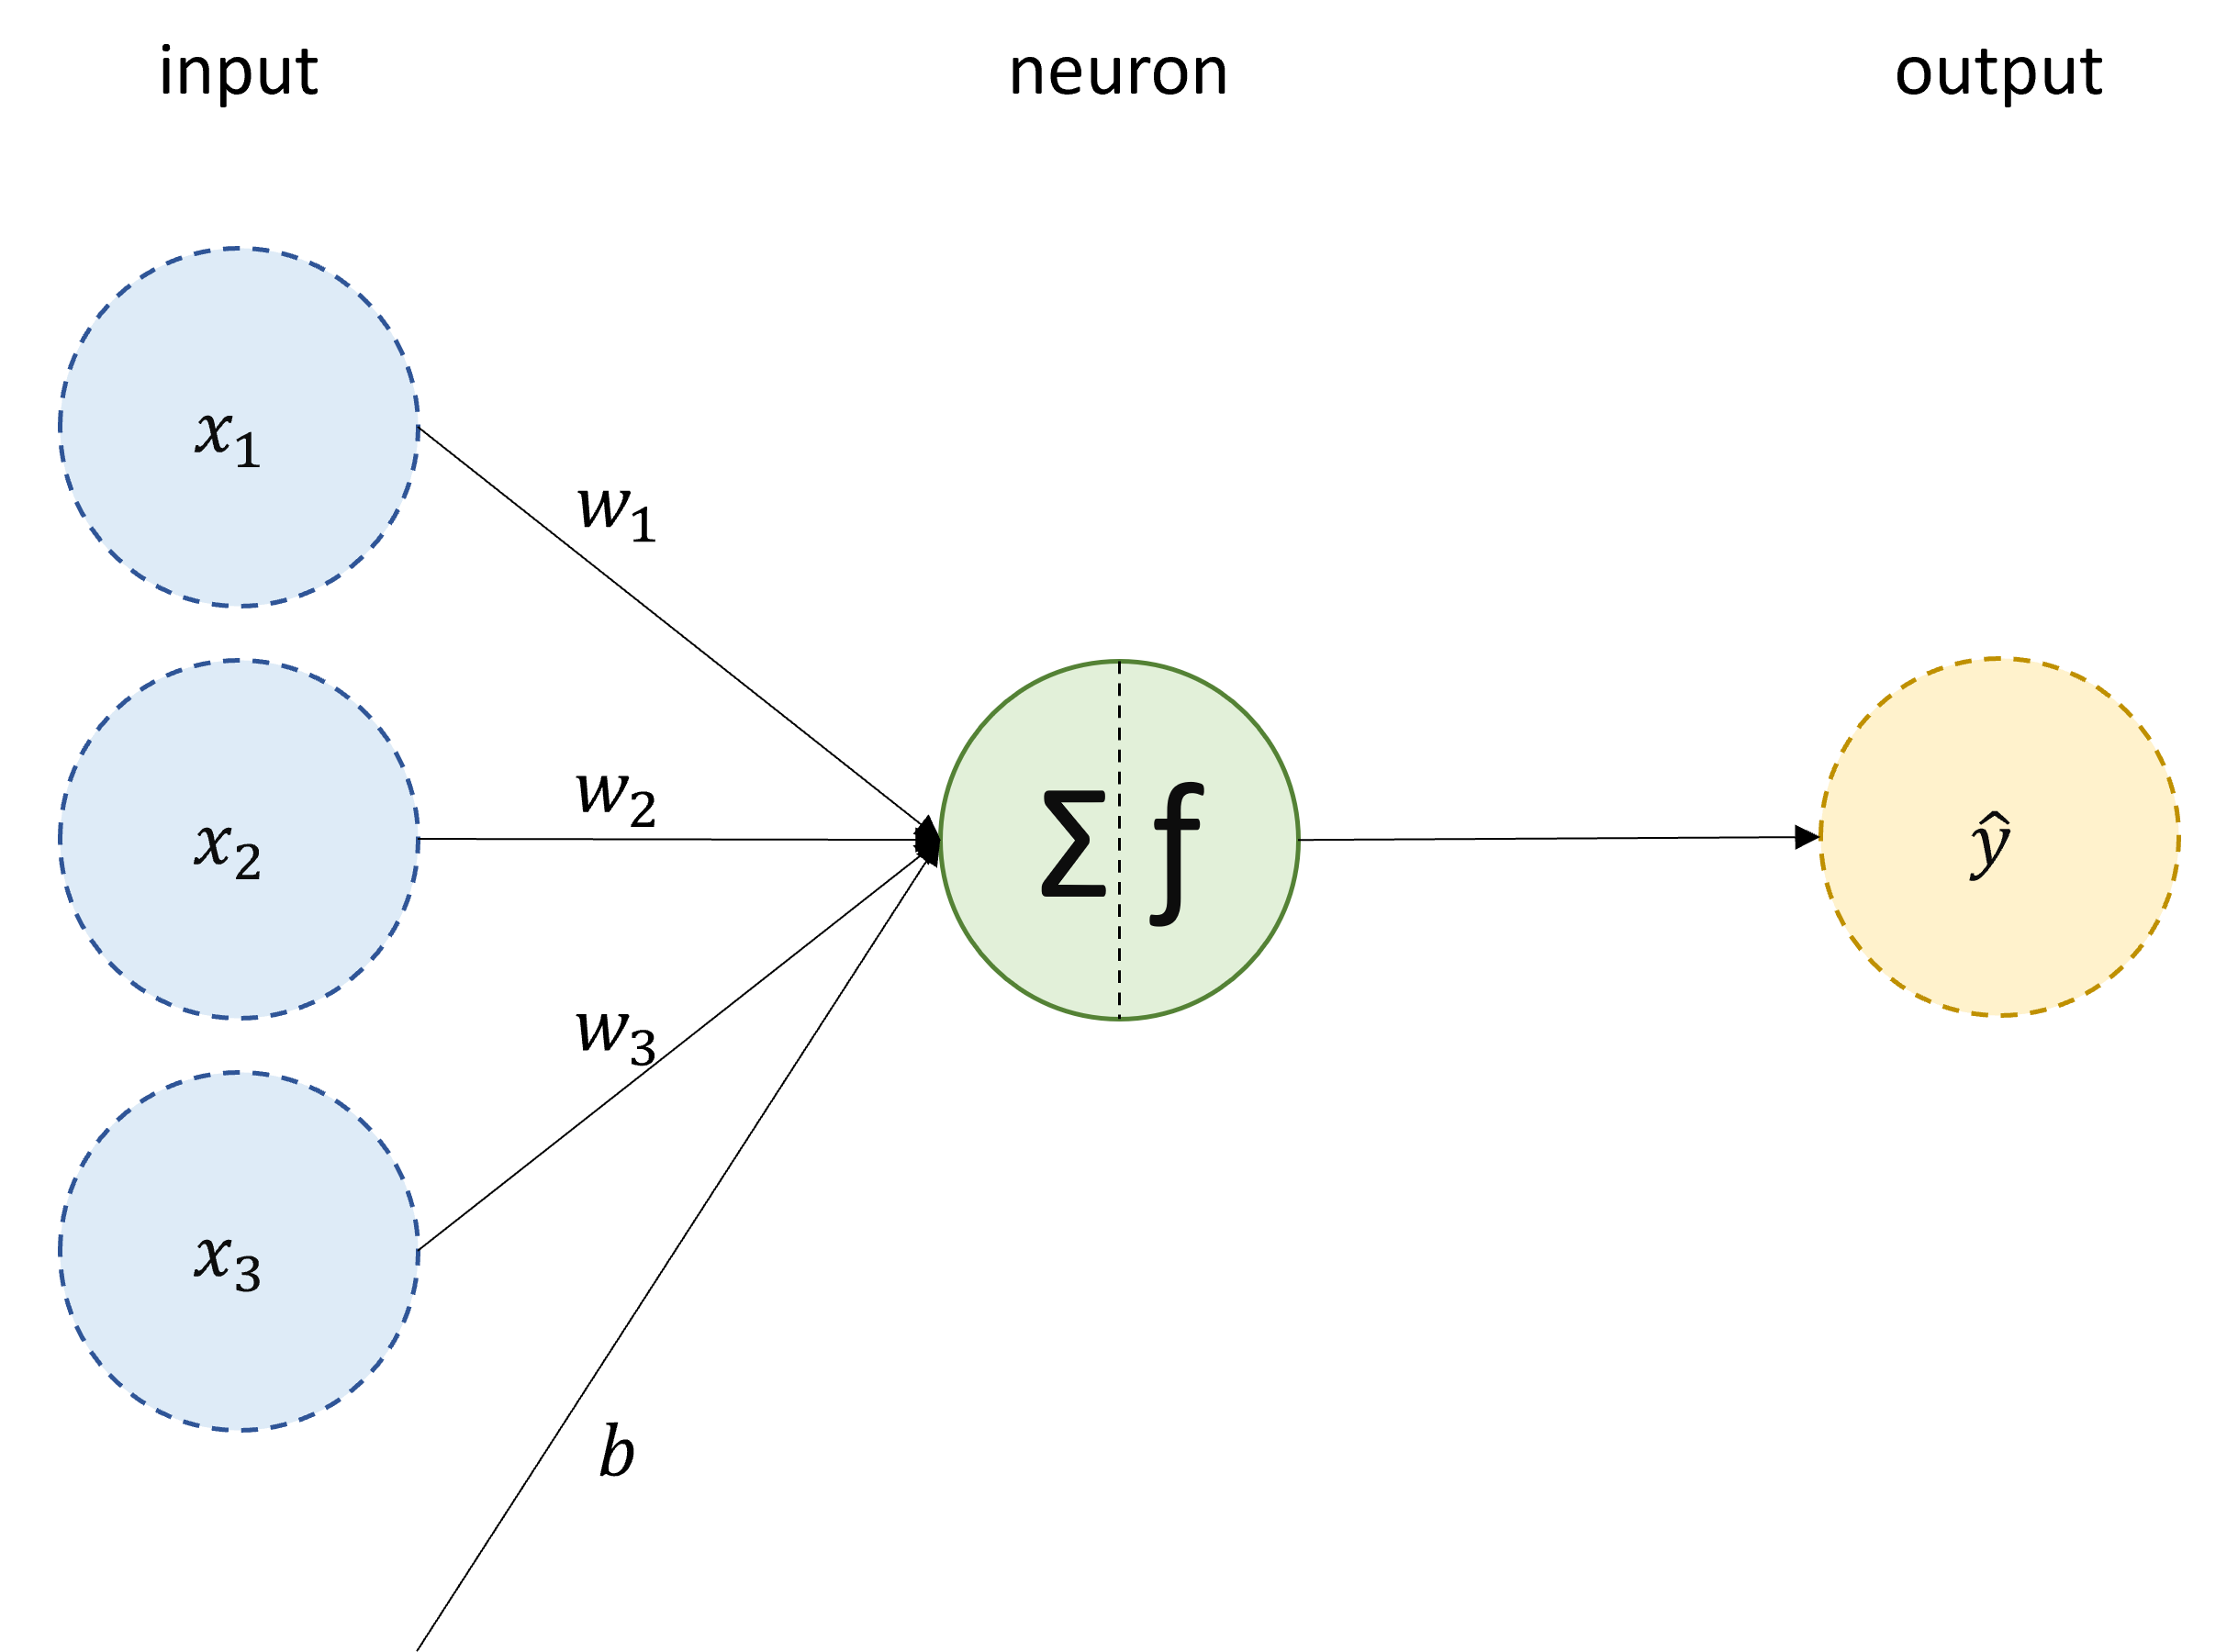
\includegraphics[width=10cm]{../images/neuron.png}
    \caption{A single neuron for binary classification}\label{fig:neuron}
    \end{center}
\end{figure}

Binary classifications usually use the sigmoid function $\sigma(z)$ as activation function to receive a fraction between 0 and 1, which can be treated as certainty. This also allows the definition of downstream threshold that favor one class to reduce type I errors.
\begin{equation}
    \sigma(z) := \frac{1}{1+e^{-z}} = \frac{e^{z}}{1+e^{z}}
\end{equation}

Classifications with more than two classes are possible by combining $K$ neurons, while $K$ is the number of classes. Thus, the weight vectors are combined in the weight matrix $\mathbf{W}$, while the biases and the outputs form the vectors $\mathbf{b}$ and $\mathbf{\hat{y}}$ respectively.
\begin{equation}
    \mathbf{W} = \begin{pmatrix}w_{1,1}&\cdots &w_{1,n}\\\vdots &\ddots &\vdots\\w_{k,1}&\cdots &w_{k,n}\end{pmatrix}\text{,}\quad\mathbf{b} = \begin{bmatrix}b_1\\\vdots \\b_k\end{bmatrix}\text{,}\quad\mathbf{\hat{y}} = \begin{bmatrix}\hat{y}_1\\\vdots \\\hat{y}_k\end{bmatrix}
\end{equation}

The softmax function is suited as activation function in such cases to produce a probability distribution as output.
\begin{equation}
    \operatorname{softmax}(\mathbf{z})_{i} := {\frac{e^{z_{i}}}{\sum_{k=1}^{K}e^{z_{k}}}}\text{ for }i=1,\dotsc ,K
\end{equation}

Figure~\ref{fig:neurons} shows such an example with four input values and three output classes.

\begin{figure}[H]
    \begin{center}
    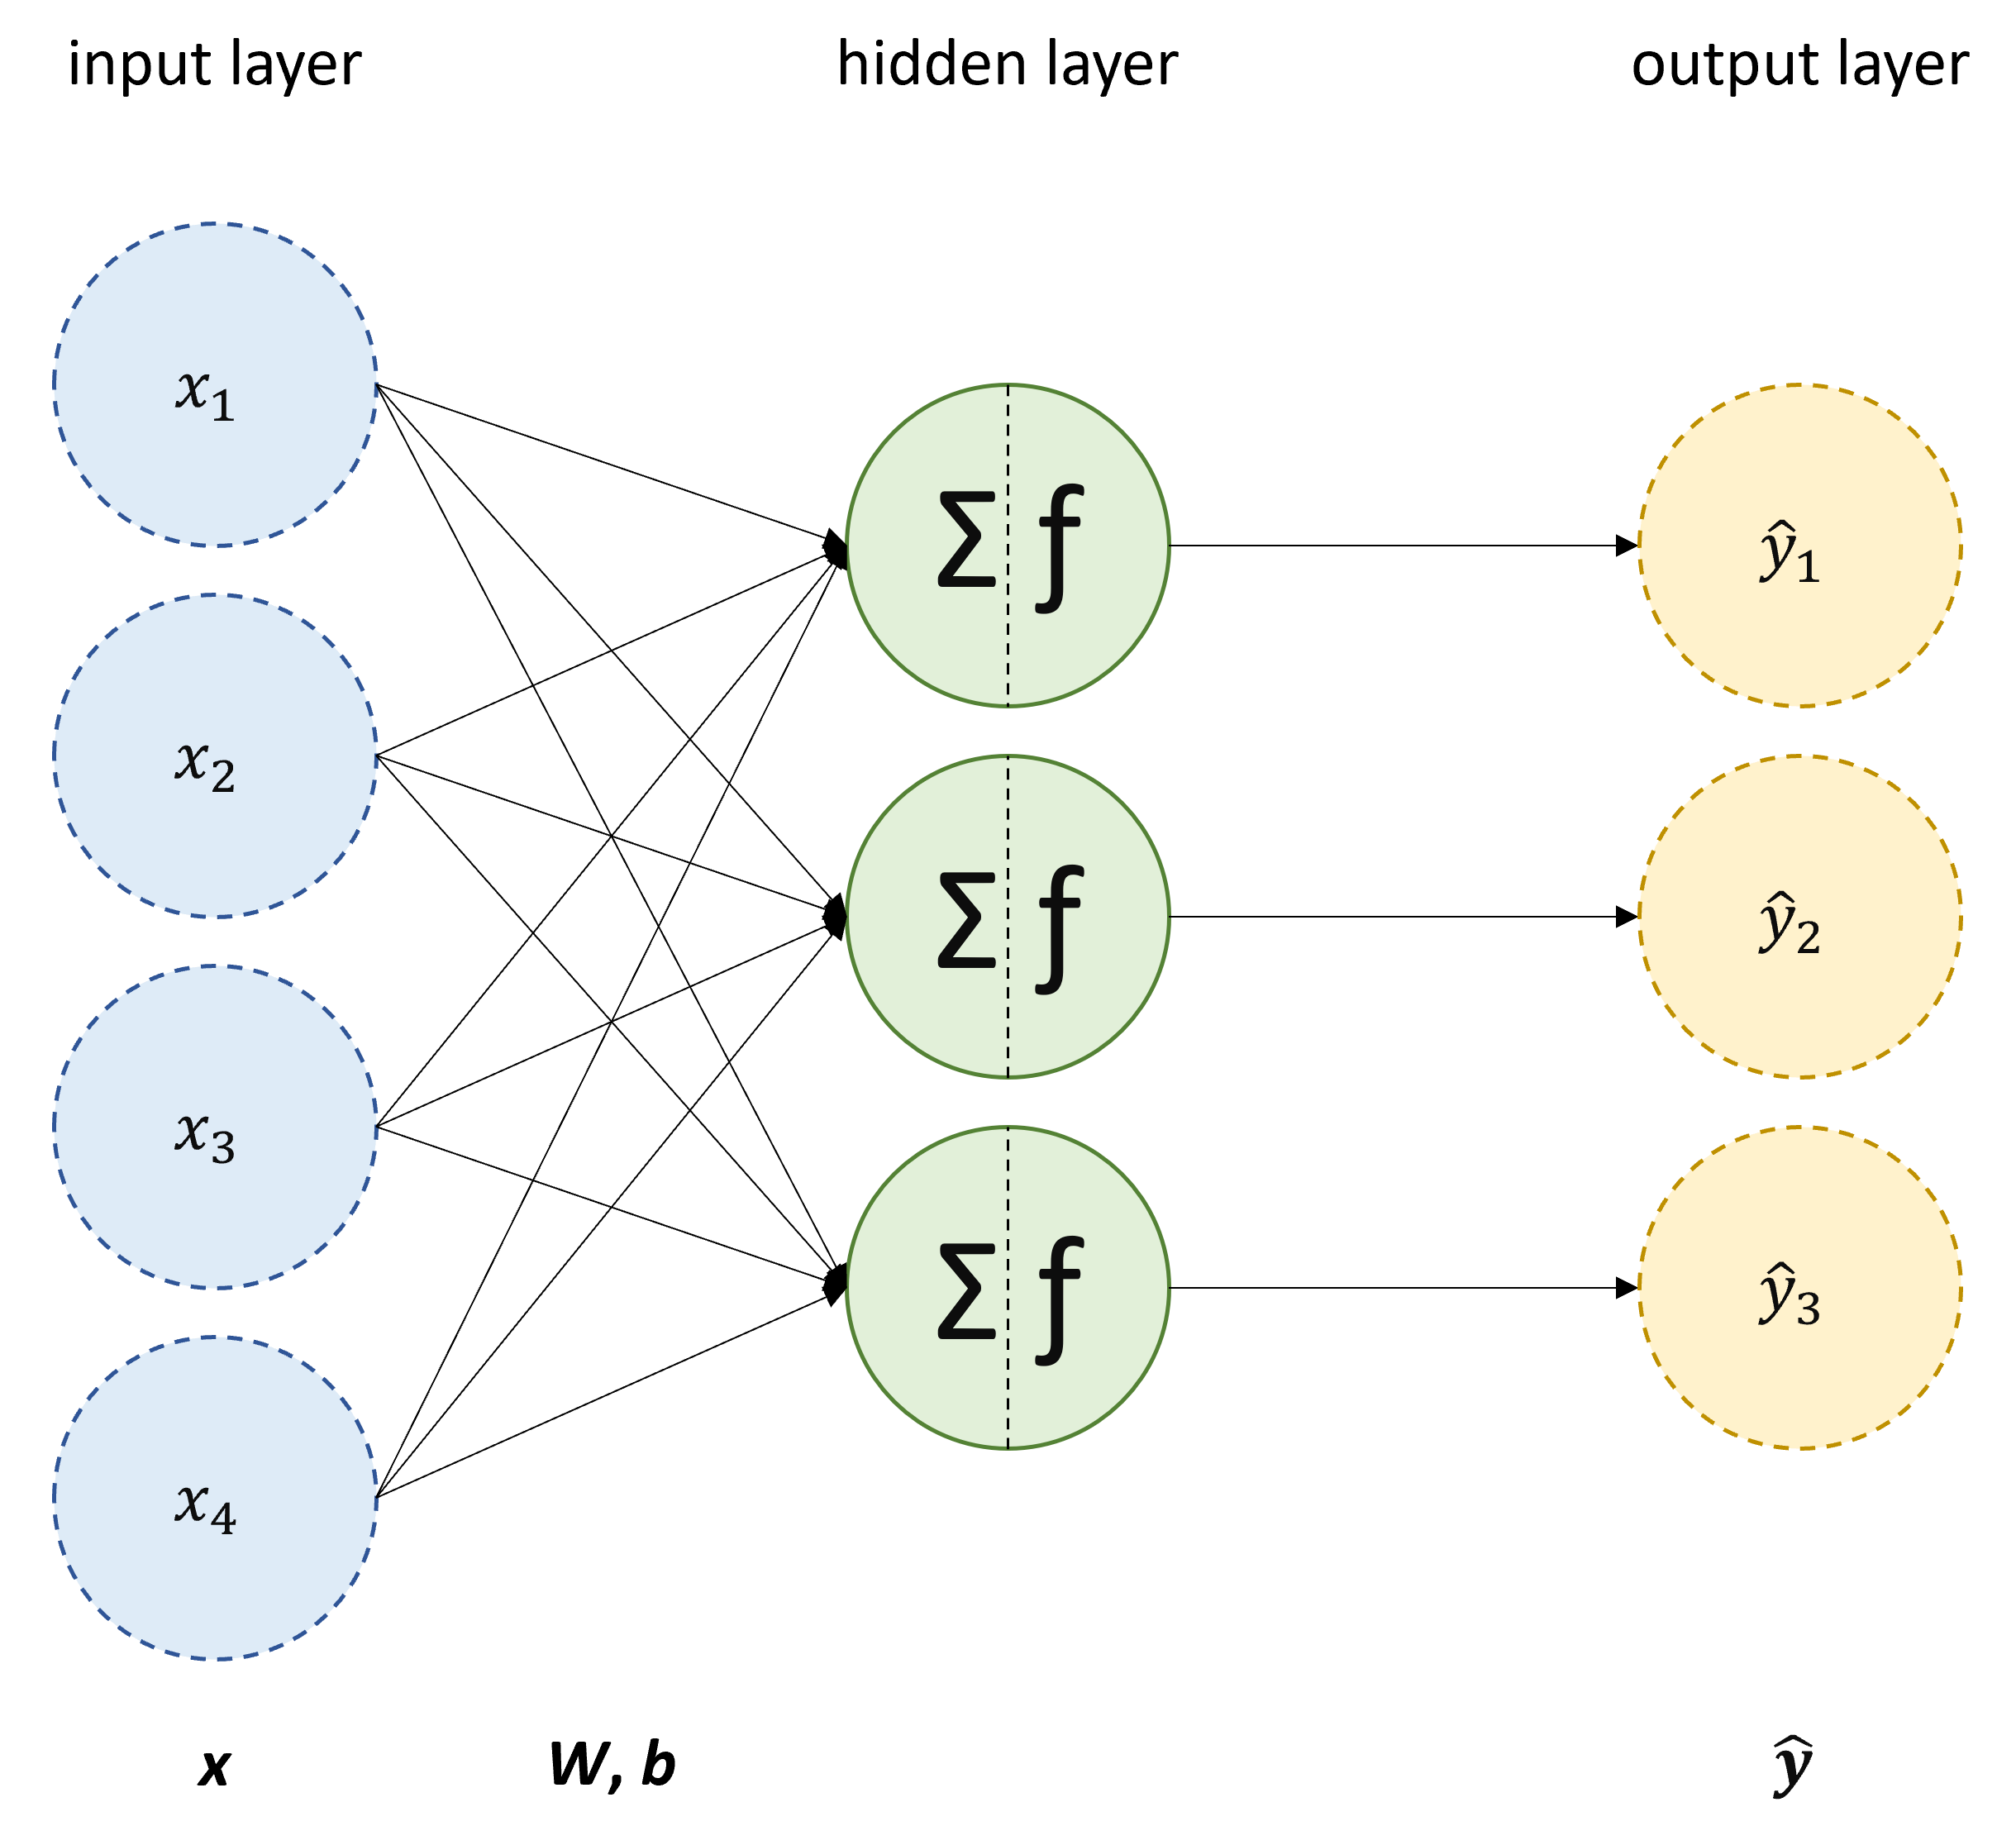
\includegraphics[width=10cm]{../images/neurons.png}
    \caption{Multiple neurons for multi class classification}\label{fig:neurons}
    \end{center}
\end{figure}

\subsection{Multilayer perceptron}
Stacking several layers of neurons leads to the \gls{mlp}. Every neuron is connected to each neuron of the previous layer making it a `dense' network.
$\sigma(z)$ and $\operatorname{softmax}(\mathbf{z})$ are computably expensive to calculate. The \gls{relu} function has a similar effect, but is much simpler and therefore better suited in all layers except the last.

\begin{equation}
\operatorname{relu}(z) := \begin{cases}z,&z>0\\0,&z\leq 0\end{cases}
\end{equation}

Figure~\ref{fig:mlp_architecture} shows the previous network with two additional hidden layers.

\begin{figure}[H]
    \begin{center}
    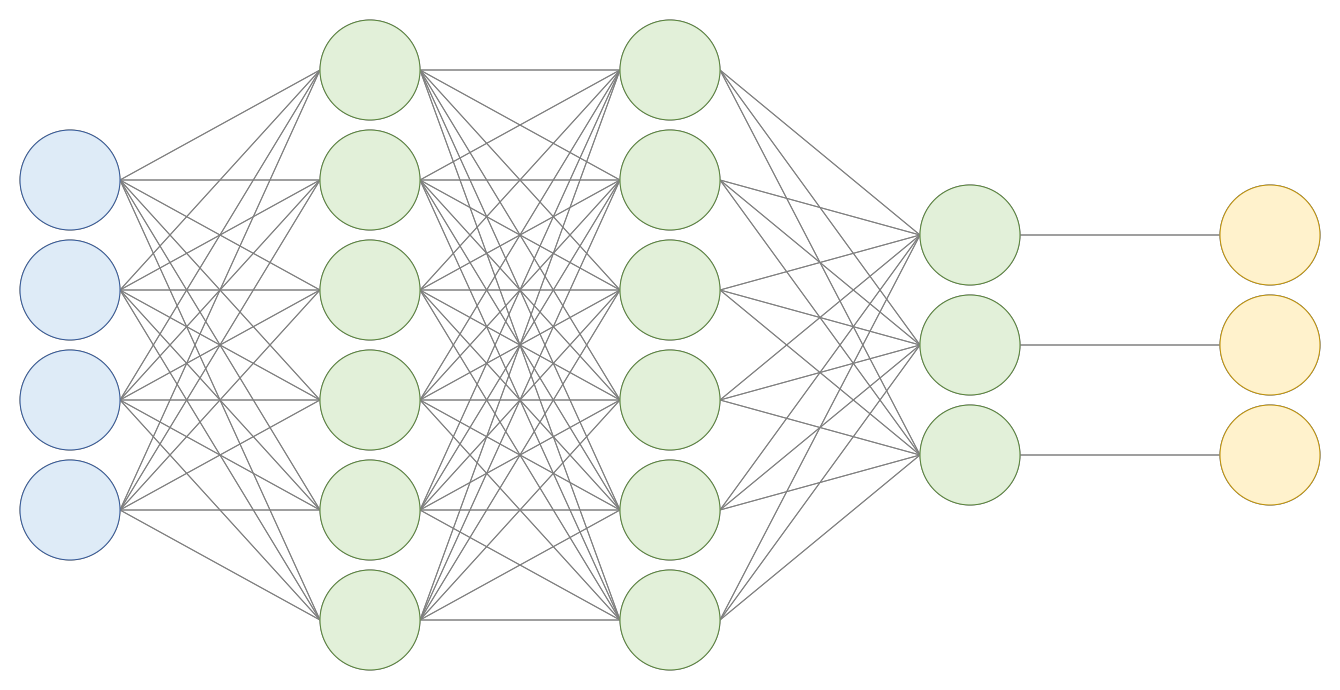
\includegraphics[width=15cm]{../images/mlp_architecture.png}
    \caption{Architecture of a basic multilayer perceptron}\label{fig:mlp_architecture}
    \end{center}
\end{figure}

% \glspl{ann} have become the de facto standard in image classification.%cite 
% The main architectures are \glspl{cnn} and the more recent \glspl{vit}.

\subsection{Convolutional neural networks}
Dense neural networks are not suited for images. Only the last few layers are usually dense to classify the extracted features. Extracting these features brings some obstacles. One one hand would a $224$ pixel high and $244$ pixel wide image already require millions of parameters per layer, which is not feasible. On the other hand should the model be resistant to small rotations and translations of the depicted object. Luckily, it is not necessary to regard all pixels in every neuron. Pixels usually highly correlate with their adjacent neighbors and therefore contain redundancy.
Filters adress these problems by combining pixels locally and extracting meaningful features per region \autocite{lecun1989}. The input data can be written as a two-dimensional matrix $\mathbf{G} \in \mathbb{R}^{w_g \times h_g}$, where $w_g$ and $h_g$ are the width and height of the input data. Every filter consists of a filter matrix $\mathbf{F} \in \mathbb{R}^{w_f \times h_f}$ and a bias scalar $b$, where $w_f$ and $h_f$ are analogously the width and height of that filter. During the `convolution' the filter is applied to the input matrix to generate the output matrix $\mathbf{O} \in \mathbb{R}^{w_o \times h_o}$.

\begin{equation}
o_{i,j} = (\mathbf{F} \ast \mathbf{G})_{i,j} = \sum_{m=1}^{w_f}\sum_{n=1}^{h_f} f_{m,n} \cdot g_{i+m, j+n} + b
\end{equation}

Depending on the values in the filter matrix $\mathbf{F}$ it is possible to carry out various operations such as finding edges or other patterns. 
Filters are usually relatively small, $3 \times 3$ pixels for example, and they use these parameters for the whole input. This ensures that the number of trainable parameters stays manageable and helps against small translations. 
Instead of producing only one output layer often multiple different filters are used on the input increasing the number of channels. 

Convolutional layers are usually alternated with pooling layers. Latters scale down the layer size and reduce the number of required neurons for classification greatly. An example of a \gls{cnn} is shown in Figure~\ref{fig:cnn_architecture}. The images is fed into the network on the left side. The convolutional layers increase the number of channels, visualized by thicker layers. The pooling layers decrease the height and width. The flattening layer concatenates all data points from the two-dimensional input batches into a one-dimensional output vector. This vector can then be used by dense layers to decrease the number of nodes to the number of classes.

\begin{figure}[H]
    \begin{center}
    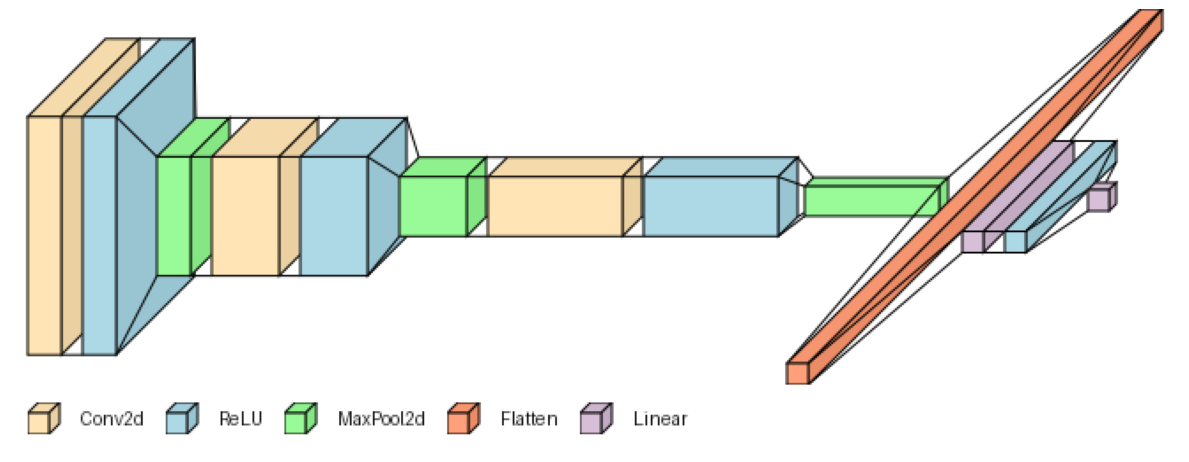
\includegraphics[width=15cm]{../images/cnn_architecture.png}
    \caption{Architecture of a basic \gls{cnn}}\label{fig:cnn_architecture}
    \end{center}
\end{figure}

\subsection{Resnet50}
Some \gls{cnn} models were able to win the ImageNet classification challenge such AlexNet \autocite{krizhevsky2012} in 2012 and \gls{vgg} \autocite{simonyan2015} in 2014. But training such deep models was laborious and reaching its limits. 

The introduction of residual connection in 2025 provided a remedy \autocite{he2015}. Residual connection copies the values of an earlier layer and adds it to a later layer. This stabilizes the training process and allows ever deeper models to be trained without vanishing gradients.
The Resnet50 architecture is one of the resulting residual neural networks, which is still widely used in image classification today. Figure~\ref{fig:resnet50_architecture} shows the structure based on the implementation from `torchvision'. Additionally, the newly discovered batch normalization is utilized to stabilize and accelerate training \autocite{ioffe2015}.

\begin{figure}[H]
    \begin{center}
    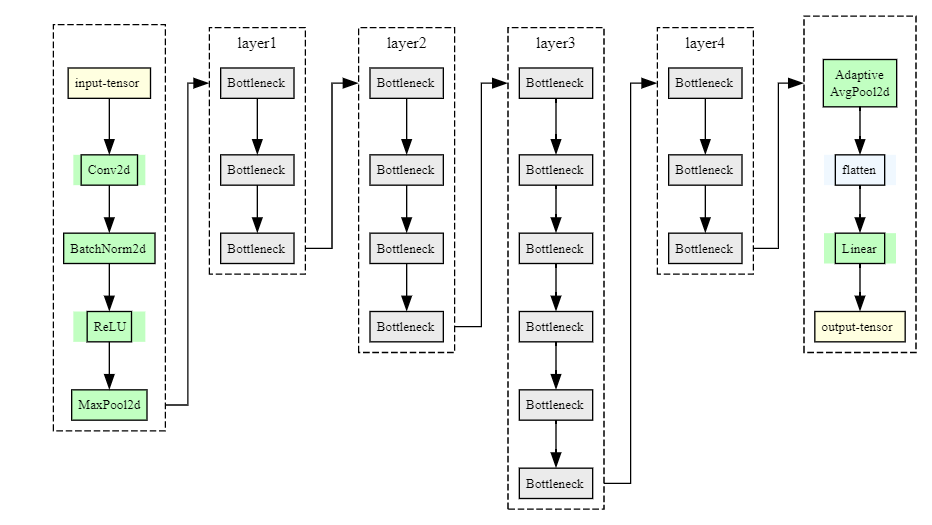
\includegraphics[width=15cm]{../images/resnet50_architecture.png}
    \caption{Architecture of Resnet50}\label{fig:resnet50_architecture}
    \end{center}
\end{figure}

Every `bottleneck' block contains the layers shown in Figure~\ref{fig:resnet50_architecture_bottleneck} including the mentioned residual connection.

\begin{figure}[H]
    \begin{center}
    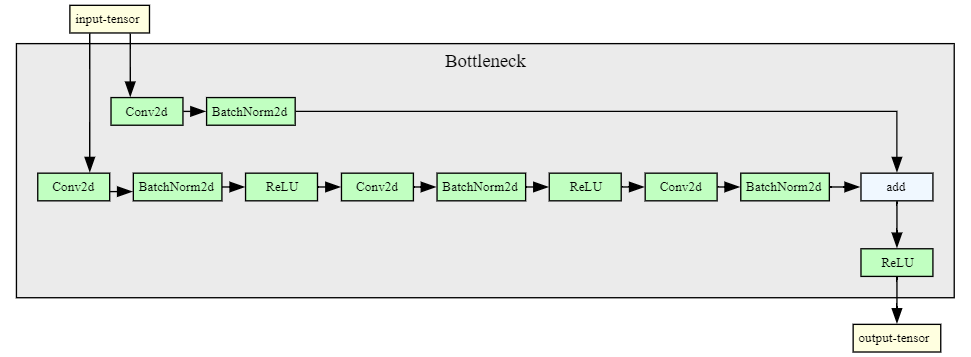
\includegraphics[width=15cm]{../images/resnet50_architecture_bottleneck.png}
    \caption{Architecture of Resnet50 bottleneck}\label{fig:resnet50_architecture_bottleneck}
    \end{center}
\end{figure}

\subsection{ViT-T/16}
Another major breakthrough was achieved 2017 by introducing the transformer \autocite{vaswani2017}. The transformer is able to handle context due to the concept of `attention'. After the broad success in \gls{nlp} transformers were introduced for visual tasks as well \autocite{dosovitskiy2020}. This original \gls{vit} comes in the sizes `base', `large' and `huge'. But further papers introduced the smaller version `tiny' \autocite{liu2021,wu2022}.

Figure~\ref{fig:vit_t16_architecture} shows the implementation of the tiny \gls{vit} in the library `timm'. Other libraries have slightly different implementations.

\begin{figure}[H]
    \begin{center}
    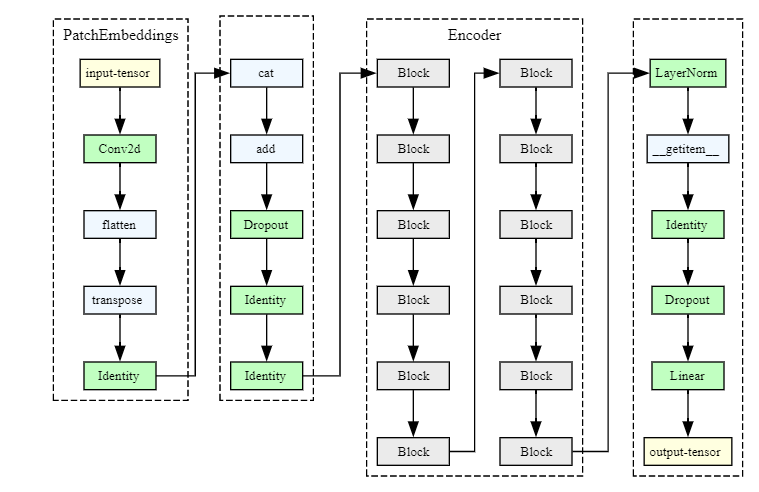
\includegraphics[width=15cm]{../images/vit_t16_architecture.png}
    \caption{Architecture of ViT-T/16}\label{fig:vit_t16_architecture}
    \end{center}
\end{figure}

Figure~\ref{fig:vit_t16_architecture_block}.

\begin{figure}[H]
    \begin{center}
    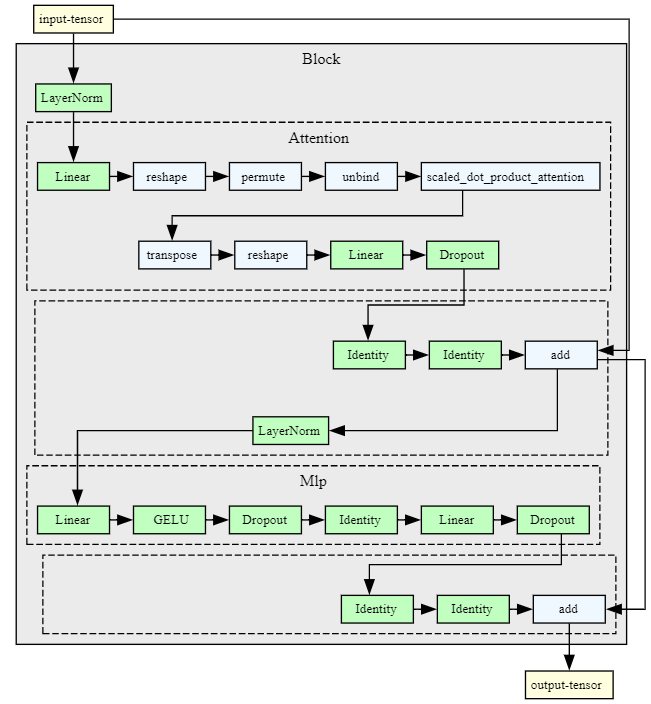
\includegraphics[width=15cm]{../images/vit_t16_architecture_block.png}
    \caption{Architecture of ViT-T/16 block}\label{fig:vit_t16_architecture_block}
    \end{center}
\end{figure}

%DINO

% AI
% Finetuning / Transfer Learning
% Modern approaches: Lora, Adapter
% Frozen evaluation
% Utility Score



% DINO
% Teacher / Student
